\documentclass[]{article}
\usepackage{geometry}[margin=1in]
\usepackage{amsmath}
\usepackage{amsfonts}
\usepackage{physics}
\usepackage{graphicx}
\usepackage{cancel}
\usepackage{setspace}
\usepackage{fancyvrb}

\setlength\parindent{0pt}

\newcommand{\sectionname}{Section}
\renewcommand{\figurename}{Fig.}

\newcommand{\Epsilon}{\mathcal{E}}

\title{MECH 6325 - Computer Assignment 1}
\author{Jonas Wagner}
\date{2020, September 28}


\begin{document}

\maketitle

\begin{abstract}
	In the assignment, a single-input single-output LTI system Transfer Function is identified given the frequency response of the system. An n-dimensional transfer function is defined and data of the the input-output frequency response of the system is used to estimate the parameters by minimizing a cost function defined by the least-squares error. The process is first derived analytically and then implemented and simulated within MATLAB.
\end{abstract}

\section*{Problem Outline}

	Let the transfer function of an LTI Transfer Function be defined as:
	\begin{align}
		G(s) &= \frac{B(s)}{A(s)}
	\end{align}
	
	with $B(s)$ and $A(s)$ defined as:
	\begin{equation}
			\begin{aligned}
			B(s) &= \sum_{i=0}^{n-1} b_i s^i = b_0 + b_1 s + b_2 s^2 + \cdots + b_{n-1}^{n-1}\\
			A(s) &= 1 + \sum_{i=1}^{n} a_i s^i = 1 + a_1 s + a_2 s^2 + \cdots + a_{n}^{n}
		\end{aligned}
		\label{eq:B(s)_A(s)_def}
	\end{equation}

	
	The input-output frequency response, $\hat{G}(j\omega)$ is calculated from the response of the system from sine waves applied to the system at different frequencies:
	\begin{align*}
		\omega = \mqty[\omega_1 \\ \omega_2 \\ \vdots\\ \omega_N]
	\end{align*}
	These measurements can then be used to estimate the actual system Transfer Function, $G(s)$.

\newpage
\section{Problem 1}
	In order to determine the optimal values for the coefficients of $A(s)$ and $B(s)$, the cost function can be defined as the sum of the squared error of the Transfer Function frequency response.\\
	Given that the frequency response of the output can be calculated as
	\begin{align}
		A(s) G(s) = B(s)
	\end{align}
	The error between the measured response and the estimate can then be calculated as:			
	\begin{align}
		\epsilon_i = A(j\omega_i) \hat{G}(j\omega_i) - B(j\omega_i)
	\end{align}
		
	By substituting in the polynomials from \eqref{eq:B(s)_A(s)_def} and defining the measured $\hat{G_i} = \hat{G}(j\omega_i)$, the error can be expanded into:
	\begin{align}
		\epsilon_i &= \hat{G}(j\omega_i) \qty(1 + \sum_{i=1}^{n} a_i s^i) - \sum_{i=0}^{n-1} b_i s^i
	\end{align}

	Next, the error can be rewritten in the least squares matrix form as follows:
	
	\begin{align}
		\Epsilon &= y - H \hat{x} \label{eq:error_def}
	\end{align}

	where,
	\begin{align}
		y &= \hat{G} = \mqty[\hat{G}_1 & \hat{G}_2 & \cdots & \hat{G}_N]^T \label{eq:y_def}\\ \nonumber\\
		\hat{x} &= \mqty[a_1 & a_2 & \cdots & a_n & b_0 & b_1 & b_2 & \cdots & b_{n-1}]^T \label{eq:x_def}
	\end{align}
	\setstretch{2}
	\begin{align}
		H &= \mqty[
					-\hat{G}_1 \ (j\omega_1) & -\hat{G}_1 \ (j\omega_1)^2 & \cdots & -\hat{G}_1 \ (j\omega_1)^n & 1 & (j\omega_1)  & \cdots &  (j\omega_1)^{n-1}\\
					-\hat{G}_2 \ (j\omega_2) & -\hat{G}_2 \ (j\omega_2)^2 & \cdots & -\hat{G}_2 \ (j\omega_2)^n & 1 & (j\omega_2)  & \cdots &  (j\omega_2)^{n-1}\\
					\vdots & \vdots & \ddots & \vdots & \vdots & \vdots  & \ddots & \vdots\\
					-\hat{G}_N \ (j\omega_N) & -\hat{G}_N \ (j\omega_N)^2 & \cdots & -\hat{G}_N \ (j\omega_N)^n & 1 & (j\omega_N) & \cdots &  (j\omega_N)^{n-1}] \label{eq:H_def}
	\end{align}
	\setstretch{1}
	
	\newpage
	The cost function used to estimate the coefficients is then defined as:
	\begin{align}
		J & = \sum_{i=1}^N \epsilon_i^* \epsilon_i = \Epsilon^* \Epsilon
	\end{align}
	
	This can then be expanded and simplified as follows:
	\begin{align}
		J = \Epsilon ^* \Epsilon 	&= \qty(y - H \hat{x})^* \qty(y - H \hat{x})\\ \nonumber
									&= y^* y - \hat{x}^* H^* y - y^* H \hat{x} + \hat{x}^* H^* H \hat{x}
	\end{align}
	
	The minimum conditions for the cost function can then be found by setting $\pdv{J}{\hat{x}} = 0$, as shown below:
	
	\begin{align}
		0 = \pdv{J}{\hat{x}} 	&= 0 -y^*H - y^* H + 2 \hat{x}^* H^* H\\
					2 y^* H		&= 2 \hat{x}^* H^* H \nonumber\\
			y^* H (H^* H)^{-1}	&= \hat{x}^* (H^* H) (H^* H)^{-1} \nonumber\\
					\hat{x}		&= (y^* H (H^* H)^{-1})^*\nonumber \\
		\intertext{	The optimal solution, $\hat{x}$, is therefore defined as:}
						\hat{x}	&= \qty(H^* H)^{-1} H^* y \label{eq:optimalSolution}
	\end{align}
	

\newpage
\section{Problem 2 - Nanopositioner Frequency Response Analysis}
	The implementation of system identification was done in MATLAB by defining an lsf() function that takes in the input and output data along with the filter order. The function then generates an H matrix and uses \eqref{eq:optimalSolution} to calculate the optimal solution. A figure is then created with a bode plot comparing the measured frequency response with the optimal solution. The lsf() function and MATLAB script can be found in Appendix \ref{apx:MATLAB}.
	
	\subsection{Guessed System Order}
		Looking at the Bode Plot of the frequency response it seemed as though the system order was 2, given the single peak and $-180 \deg$ \ steady-state phase response. This was implemented and the results for the second order system can be seen in \figurename \ref{fig:pblm2_n=2}.
	
		\begin{figure}[h]
			\centering
			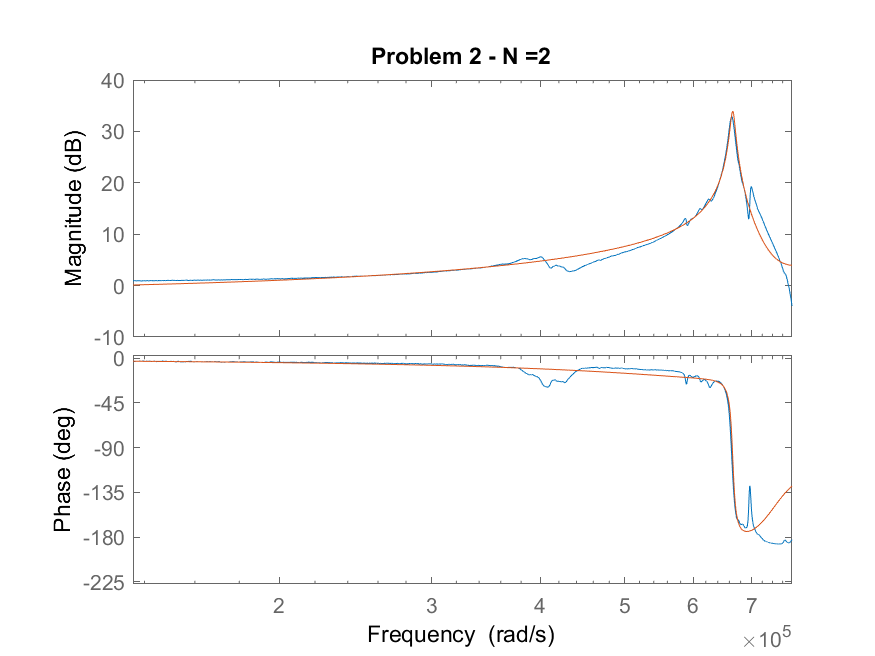
\includegraphics[width=0.7\linewidth]{fig/MECH6325_CA1_pblm2_n=2}
			\caption{Bode Plot of the measured response of the nanopositioner versus the second order least-squares estimated system.}
			\label{fig:pblm2_n=2}
		\end{figure}
		
	\subsection{Higher Order System Comparison}
		The initial estimate appears to be effectively close to the measured data, but doesn't appear to capture all of the features of the response. Higher order systems were then also computed and plotted. \figurename \ref{fig:pblm2_n=357} shows the response for the third, fifth, and seventh order systems. As can be seen, the third and fifth order estimates appear to align well with the measured data and are generally close fits then the secound order systems; however, the seventh order system (and even some other higher order) system responses appear to diverge from the measured data at higher frequencies. Additional orders of estimates can be seen in Appendix \ref{apx:figs}.
		
		\begin{figure}
			\centering
			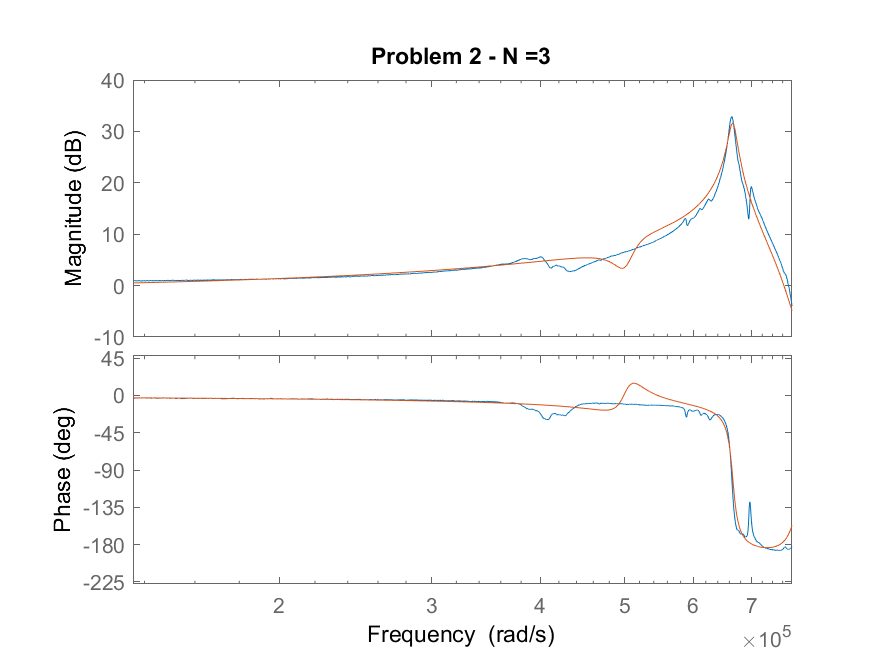
\includegraphics[width=0.6\linewidth]{fig/MECH6325_CA1_pblm2_n=3}
			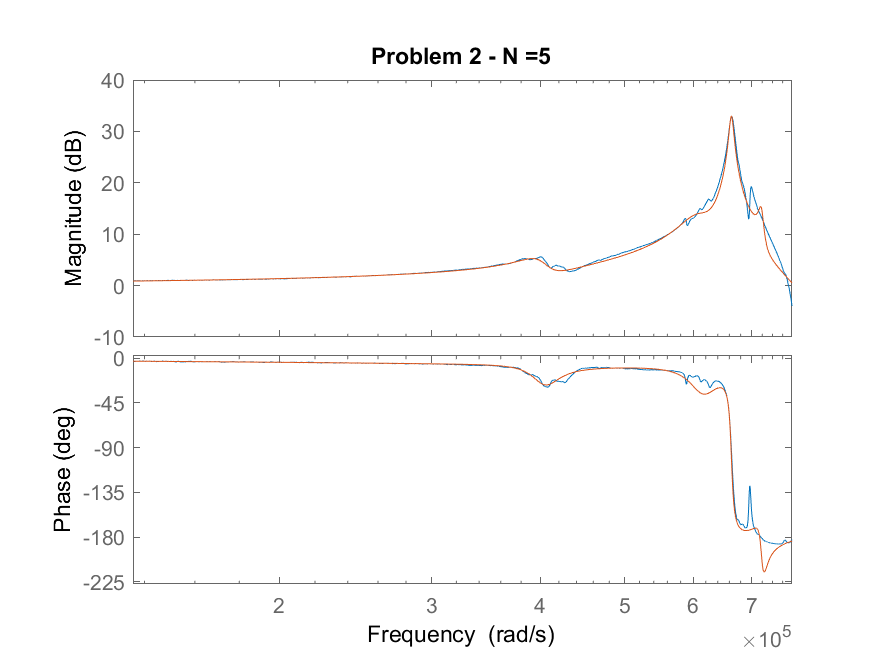
\includegraphics[width=0.6\linewidth]{fig/MECH6325_CA1_pblm2_n=5}
			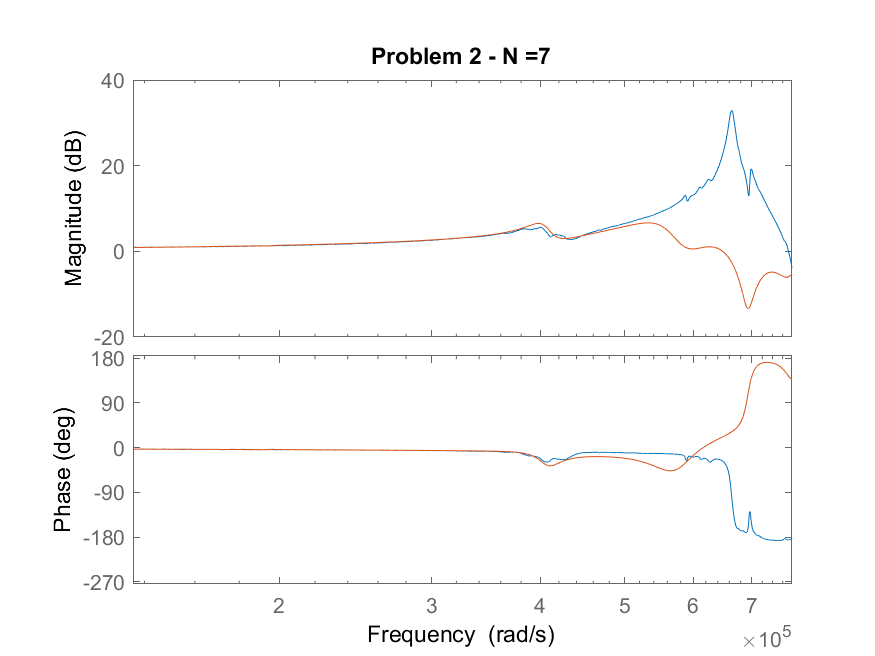
\includegraphics[width=0.6\linewidth]{fig/MECH6325_CA1_pblm2_n=7}
			\caption{Bode Plot of the measured response of the nanopositioner versus least-squares estimated systems of higher order.}
			\label{fig:pblm2_n=357}
		\end{figure}

\newpage
\section{Problem 3: Cantilever Beam Mode Analysis}
	For analyzing the second set of data, a similar process was used. The same lsf() function was used and similar bode plots were used to compare with the measured response.
	\subsection{Guessed System Order}
		The bode plot of the measured frequency response appeared to have 3 peaks, 2 troughs, and maintained a negative 20 db/decade at the end, leading me to guess a system order of 7. The seventh order system response can been seen in \figurename \ \ref{fig:pblm3_n_7}. This appears to be a good fit to the measured system response (although the phase does get plotted off by 2 Pi for some reason).

		\begin{figure}[h]
			\centering
			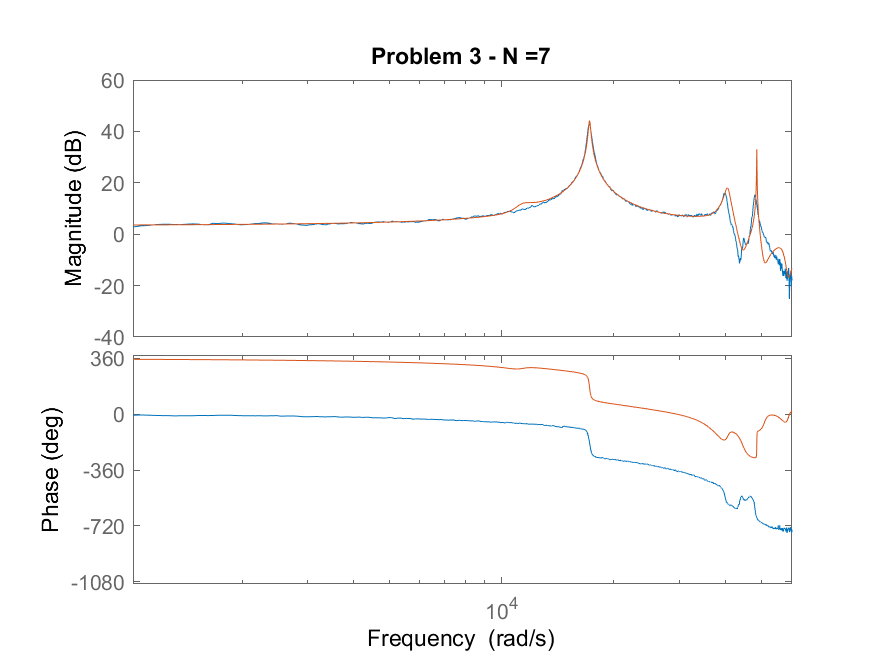
\includegraphics[width=0.75\linewidth]{fig/MECH6325_CA1_pblm3_n=7}
			\caption{Bode Plot of the measured response for the cantilever beam versus the seventh order least-squares estimated system.}
			\label{fig:pblm3_n_7}
		\end{figure}
	
	\subsection{Higher Order System Comparison}
		Similarly to how the higher order systems of the nanopositioners estimates, the fit improved for slightly higher-order systems, but untimely diverged at higher frequencies when the order continued increasing. As shown in the bode plots within \figurename \ \ref{fig:pblm3_n=81011}, the 8th order system was a better fit then the 7th order, (especially noticeable at higher frequencies), but the 10th and 12th order systems clearly diverge at the higher frequencies. Additional plots can be seen in Appendix \ref{apx:figs}.
		
	
		\begin{figure}
			\centering
			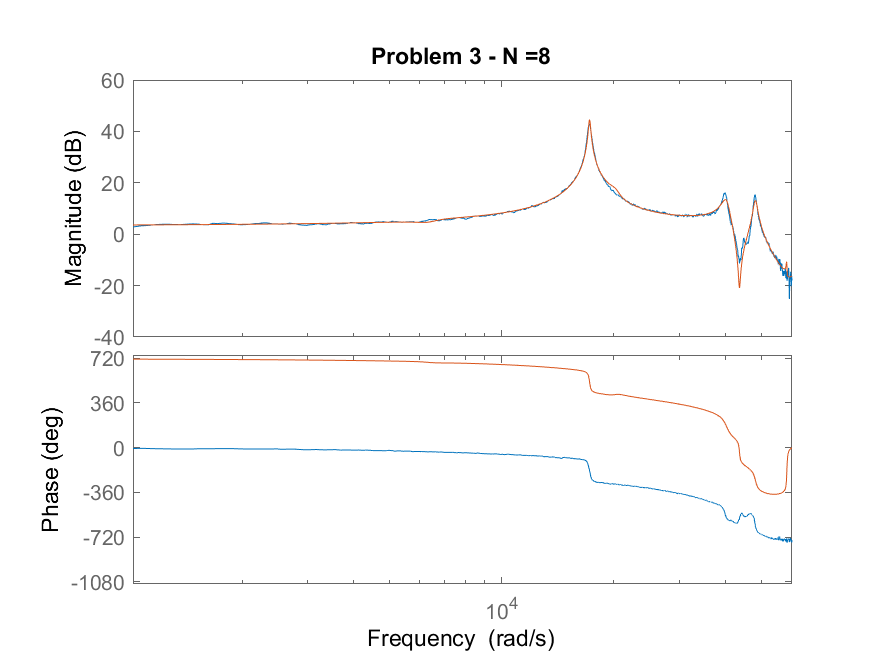
\includegraphics[width=0.6\linewidth]{fig/MECH6325_CA1_pblm3_n=8}
			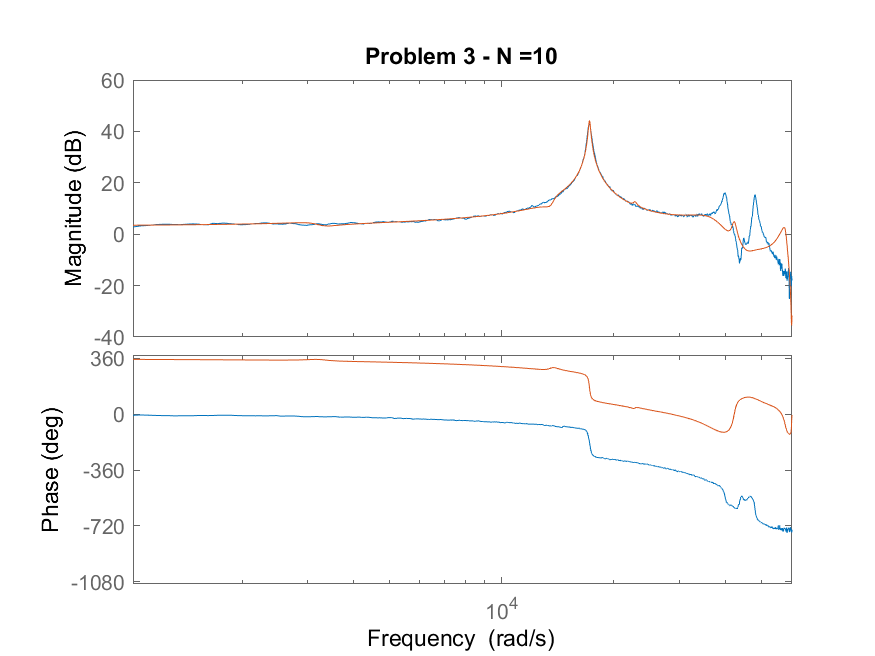
\includegraphics[width=0.6\linewidth]{fig/MECH6325_CA1_pblm3_n=10}
			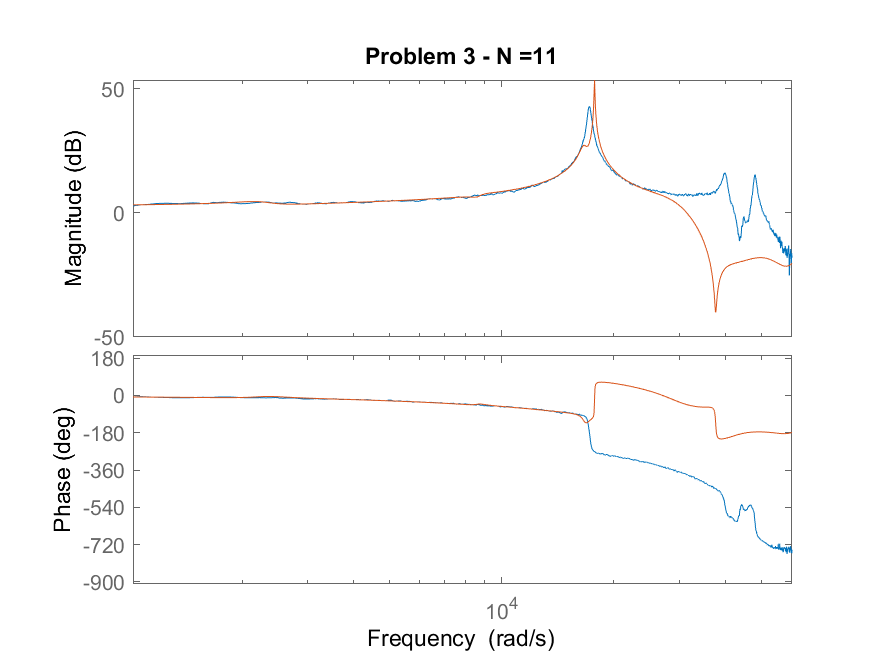
\includegraphics[width=0.6\linewidth]{fig/MECH6325_CA1_pblm3_n=11}
			\caption{Bode Plot of the measured response of the cantilever beam versus least-squares estimated systems of higher order.}
			\label{fig:pblm3_n=81011}
		\end{figure}
	
	\newpage
	\subsection{Weighting Function Implementation}
		In order to improve the fit of the least-squares estimate to the actual system response, a method that attempts to eliminate the noise is needed. A weighting function is easy to implement when the uncertainty of each measurement is explicitly known; however, the uncertainty of measurements for this data is not known. It is possible to make the assumption that uncertainty is a function of frequency, however if it is white noise is assumed, this does not exist. One potential method of generating uncertainty is to compare each data point to a windowed mean, however this may actually have the reverse effect and cause the higher frequencies to have a worse fit. Either way, the process of implementing weighted least-squares algorithm remains the same:
		
		First, in addition to the definitions from \eqref{eq:error_def}, \eqref{eq:y_def}, \eqref{eq:x_def}, and \eqref{eq:H_def}, let the following be defined as:
		
		\begin{align}
			v &= \mqty[v_1	&v_2	&\cdots	&v_N]^T\\ \nonumber\\
			R &= E[v v^T] = \mqty[	\sigma_1^2	&\cdots	&0\\
									\vdots		&\ddots	&\vdots\\
									0			&\cdots	&\sigma_N^2
									]\\ \nonumber \\
			J &= \Epsilon^* R^{-1} \Epsilon\\
			  &= (y - H\hat{x})^* R^{-1} (y - H\hat{x})\nonumber\\
			  &= y^*R^{-1}y - \hat{x}^T H^* R^{-1} y - y^* R^{-1} H \hat{x} + \hat{x}^T H^* R^{-1} H \hat{x}\nonumber
		\end{align}
		
		The optimal solution can then be derived by minimizing the cost function:
		\begin{align}
			\dv{J}{\hat{x}} = 0 &= -y^* R^{-1} H + \hat{x}^T H^* R^{-1} H\\
			H^* R^{-1} y &= H^* R^{-1} H \hat{x} \nonumber\\
		\intertext{This reults in the optimal solution defined as:}
			\hat{x} &= (H^* R^{-1} H)^{-1} H^* R^{-1} y
		\end{align}
	
		Using this optimal solution, this can then be implemented by modifying the lsf() function to include an $R$ matrix that will result in a weighted fit.
	
	\subsection{Limited Data Least-Squares}
		Selecting a subset of data will provide less information for a least-squares estimate to use to create a good fit. A smart selection may make it possible to have an acceptable estimate. In order to test this, the same lsf() function was used and provided with various subsets of the data. In general, the fits were not very great and untimely this proved that the best way to fit the data was to ensure that there is enough data provided for regions that are of interest. Two fits that appeared to be fairly acceptable are shown in \figurename \ref{fig:pblm3_iv}. Depending on the range of operation, these fits may be perfectly acceptable. Each subset contains about 75\% of the original response data. That attached MATLAB script will produce a wide range of bode plots for different subsets of data, but as each subset gets smaller the frequency range it is an acceptable fit for decreases.
		
		\begin{figure}[h]
			\centering
			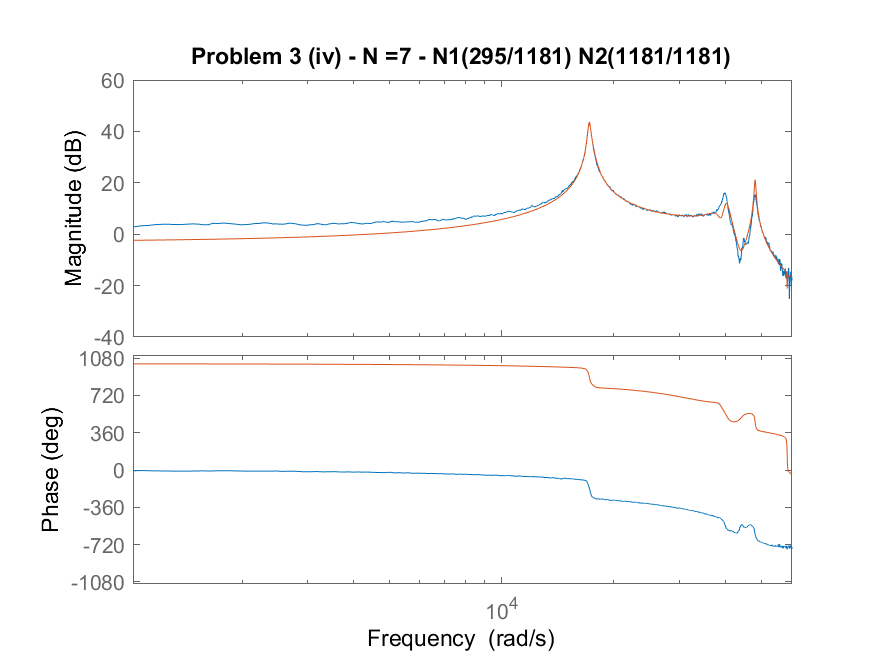
\includegraphics[width=0.6\linewidth]{fig/MECH6325_CA1_pblm3_iv_n=7N1(4)N2(0)}
			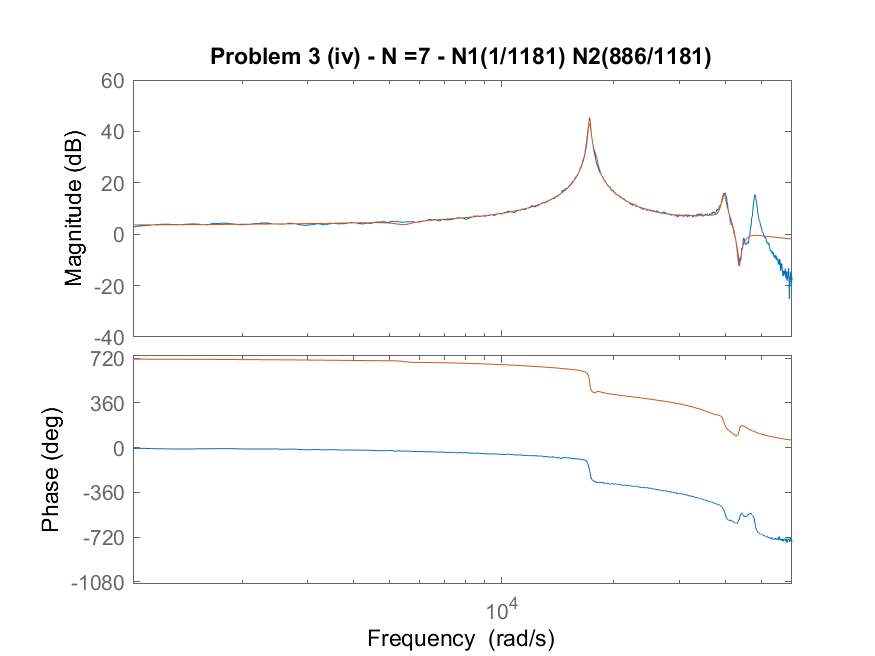
\includegraphics[width=0.6\linewidth]{fig/MECH6325_CA1_pblm3_iv_n=7N1(0)N2(4)}
			\caption{Frequency response of a least-squares estimate using subsets of data.}
			\label{fig:pblm3_iv}
		\end{figure}
		
	
\newpage
\appendix
\section{MATLAB Code} \label{apx:MATLAB}

	\subsection{lsf() Function}
		\begin{Verbatim}[tabsize=4]
		function [H, x, num, den] = lsf(n,N,u,y)
			H = zeros(N,n);
			for i = 1:n
				for k = 1:N
					H(k,i) = -y(k)* (1i * u(k))^i;
				end
			end
			
			for i = 0:(n-1)
				for k = 1:N
					H(k,i+n+1) = (1i * u(k))^i;
				end
			end
			
			x = inv(H' * H) * H' * y;
			
			
			num = fliplr(x(n+1:end).');
			den = fliplr([1, x(1:n).']);
		end
		\end{Verbatim}
		
	\subsection{MATLAB Script}
	
		\begin{Verbatim}
	clear
	close all
	clc
	
	%---------------------------------------------------------------------
	%Problem 2
	
	% vector fresp contains (complex-valued) frequency responses
	% vector w, contains frequencies at which measurements were taken
	
	load G11QA1.mat
	fresp=Yo2i(1:end);
	
	%frequency vector (in Hz)
	freq=Yo2ix(1:end);
	
	%frequency vector (in rad/sec)
	w = 2*pi*freq;
	
	%non-parametric model
	G_h = frd(fresp,w);
	
	N = length(w);
	
	y = fresp(1:N);
	u = w(1:N);
	
	% (i) Order Guess
	n = 2;
	
	[~, ~, num, den] = lsf(n,N,u,y);
	G = tf(num,den);
	
	figure()
	bode(G_h,w)
	hold on
	bode(G,w)
	title("Problem 2 - N =" + string(n))
	hold off
	
	saveas(gcf,"fig/MECH6325_CA1_pblm2_n=" + string(n) + ".png")
	
	% (ii) Higher Orders
	
	for i = (n+1):(n+5)
		n = i;
		[~, ~, num, den] = lsf(n,N,u,y);
		G = tf(num,den);
		
		figure()
		bode(G_h,w)
		hold on
		bode(G,w)
		title("Problem 2 - N =" + string(n))
		hold off
		saveas(gcf,"fig/MECH6325_CA1_pblm2_n=" + string(n) + ".png")
	end
	
	close all
	
	
	%---------------------------------------------------------------------
	%Problem 3
	
	% vector fresp contains (complex-valued) frequency responses
	% vector w, contains frequencies at which measurements were taken
	
	load G11QA2.mat
	fresp=o2i1(20:1200);%frequency response vector
	
	%frequency vector (in Hz)
	freq=o2i1x(20:1200);
	
	%frequency vector (in rad/sec)
	w = 2*pi*freq;
	
	%non-parametric model
	G_h = frd(fresp,w);
	
	N = length(w);
	
	y = fresp(1:N);
	u = w(1:N);
	
	% (i) Order Guess
	n = 7;
	
	[~, ~, num, den] = lsf(n,N,u,y);
	G = tf(num,den);
	
	figure()
	bode(G_h,w)
	hold on
	bode(G,w)
	title("Problem 3 - N =" + string(n))
	hold off
	
	saveas(gcf,"fig/MECH6325_CA1_pblm3_n=" + string(n) + ".png")
	
	% (ii) Higher Orders
	
	for i = (n+1):(n+5)
		n = i;
		[~, ~, num, den] = lsf(n,N,u,y);
		G = tf(num,den);
		
		figure()
		bode(G_h,w)
		hold on
		bode(G,w)
		title("Problem 3 - N =" + string(n))
		hold off
		saveas(gcf,"fig/MECH6325_CA1_pblm3_n=" + string(n) + ".png")
	end
	
	close all
	
	
	% (iv) Subset of data tests
	
	Nmax = N;
	
	for i = 0:4
		for j =0:4
			if i > 0
				N1 = int32(Nmax/i);
			else
				N1 = 1;
			end
			if j > 0
				N2 = Nmax - int32(Nmax/j);
			else
				N2 = Nmax;
			end
			
			if N2 > N1
				N = N2-N1 +1;
				
				y = fresp(N1:N2);
				u = w(N1:N2);
				
				n = 7;
				[~, ~, num, den] = lsf(n,N,u,y);
				G = tf(num,den);
				
				figure()
				bode(G_h,w)
				hold on
				bode(G,w)
				title("Problem 3 (iv) - N =" + string(n) + " - N1(" + string(N1) + "/" + string(Nmax) +") N2(" + string(N2) + "/" + string(Nmax)+")")
				hold off
				saveas(gcf,"fig/MECH6325_CA1_pblm3_iv_n=" + string(n) + "N1(" + string(i) + ")N2(" + string(j) + ")" + ".png")
			end
		end
	end
		\end{Verbatim}
	
	
	

\newpage
\section{Additional Figures}\label{apx:figs}
		
		\begin{figure}[h]
			\centering
			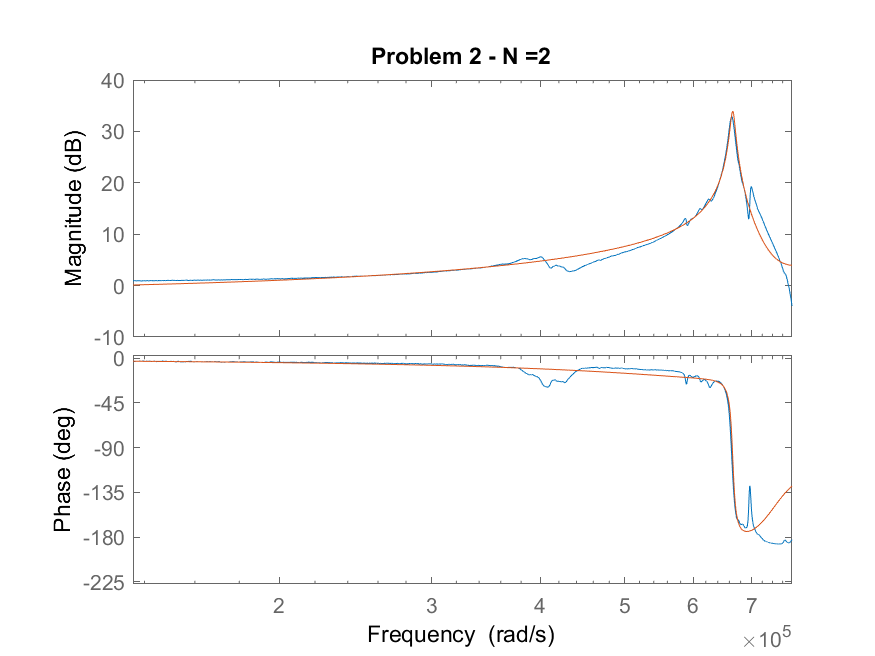
\includegraphics[width=0.7\linewidth]{fig/MECH6325_CA1_pblm2_n=2}
			\caption{Bode Plot of the measured response versus the second order least-squares estimated system.}
			\label{fig:pblm2_n=2e}
		\end{figure}
	
		\begin{figure}[h]
			\centering
			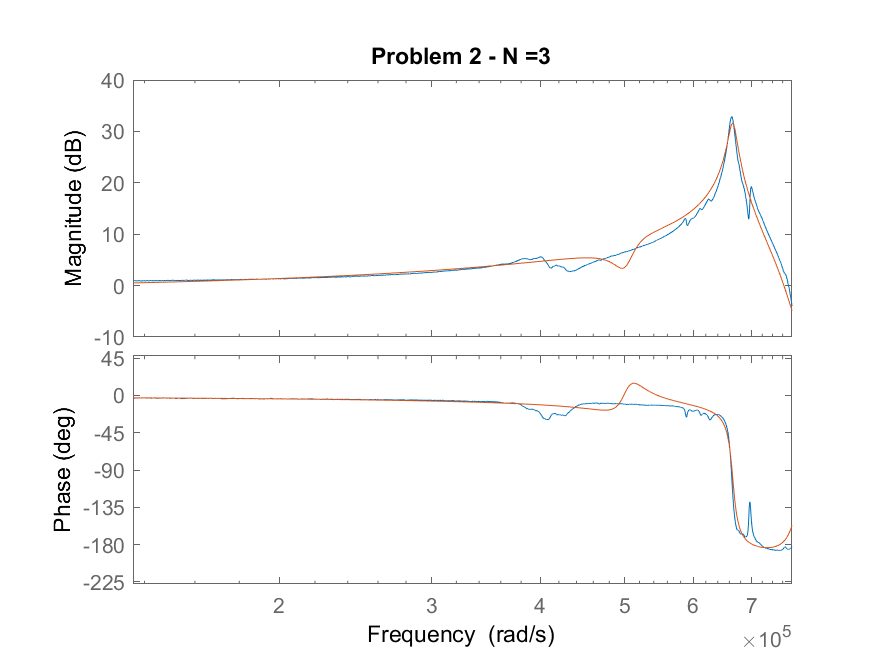
\includegraphics[width=0.7\linewidth]{fig/MECH6325_CA1_pblm2_n=3}
			\caption{Bode Plot of the measured response versus the 3rd order least-squares estimated system.}
			\label{fig:pblm2_n=3}
		\end{figure}

		\begin{figure}[h]
			\centering
			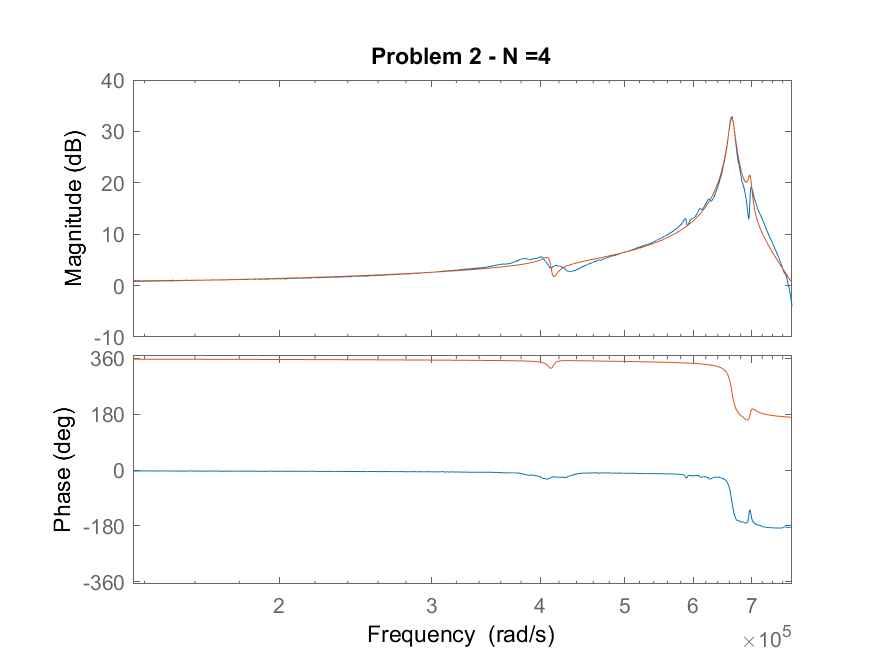
\includegraphics[width=0.7\linewidth]{fig/MECH6325_CA1_pblm2_n=4}
			\caption{Bode Plot of the measured response versus the 4th order least-squares estimated system.}
			\label{fig:pblm2_n=4}
		\end{figure}

		\begin{figure}[h]
			\centering
			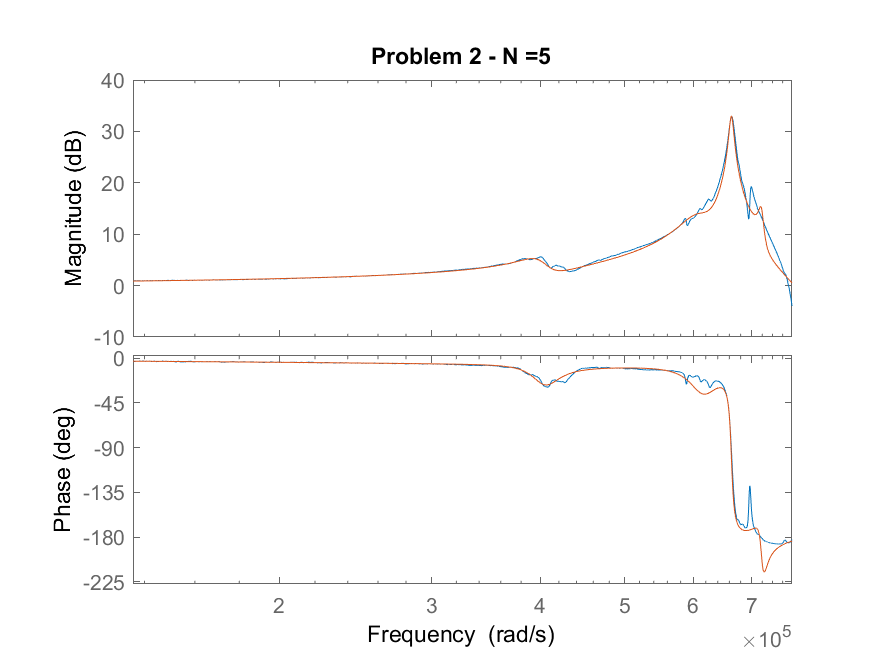
\includegraphics[width=0.7\linewidth]{fig/MECH6325_CA1_pblm2_n=5}
			\caption{Bode Plot of the measured response versus the 5th order least-squares estimated system.}
			\label{fig:pblm2_n=5}
		\end{figure}

		\begin{figure}[h]
			\centering
			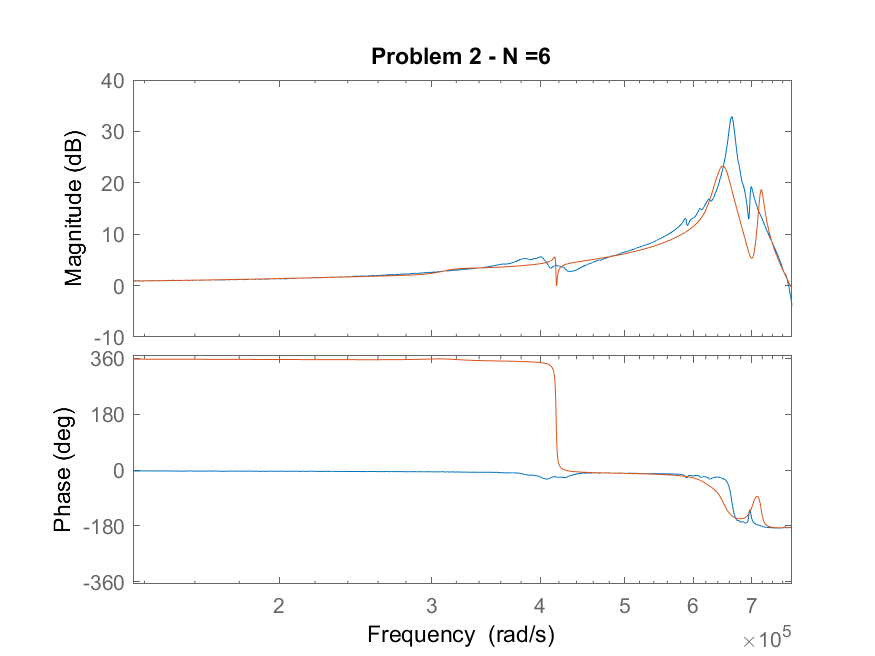
\includegraphics[width=0.7\linewidth]{fig/MECH6325_CA1_pblm2_n=6}
			\caption{Bode Plot of the measured response versus the 6th order least-squares estimated system.}
			\label{fig:pblm2_n=6}
		\end{figure}

		\begin{figure}[h]
			\centering
			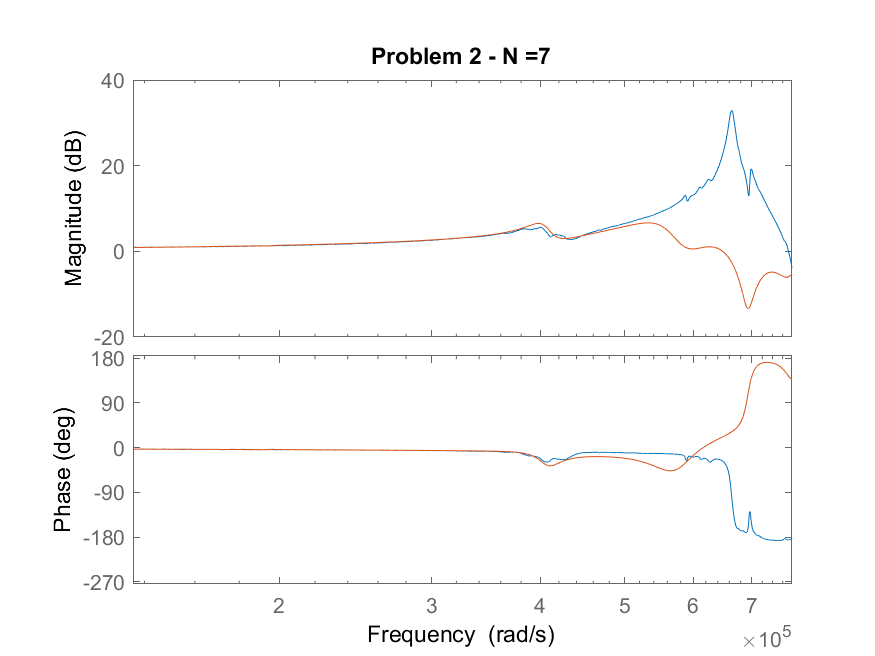
\includegraphics[width=0.7\linewidth]{fig/MECH6325_CA1_pblm2_n=7}
			\caption{Bode Plot of the measured response versus the 7th order least-squares estimated system.}
			\label{fig:pblm2_n=7}
		\end{figure}
		
		
		\begin{figure}[h]
			\centering
			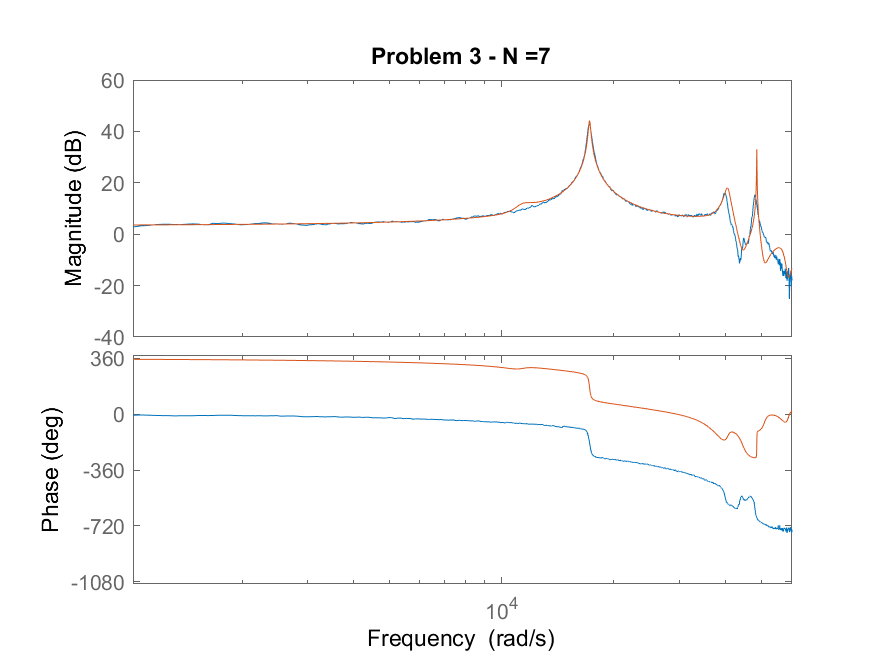
\includegraphics[width=0.7\linewidth]{fig/MECH6325_CA1_pblm3_n=7}
			\caption{Bode Plot of the measured response versus the 7th order least-squares estimated system.}
			\label{fig:pblm3_n=7}
		\end{figure}
		
		\begin{figure}[h]
			\centering
			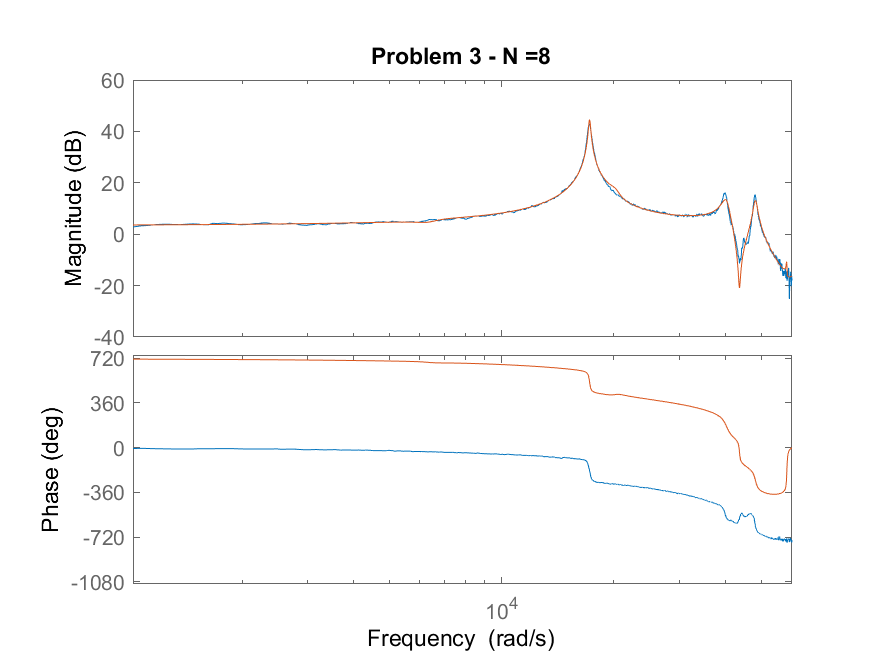
\includegraphics[width=0.7\linewidth]{fig/MECH6325_CA1_pblm3_n=8}
			\caption{Bode Plot of the measured response versus the 8th order least-squares estimated system.}
			\label{fig:pblm3_n=8}
		\end{figure}
	
		\begin{figure}[h]	
			\centering
			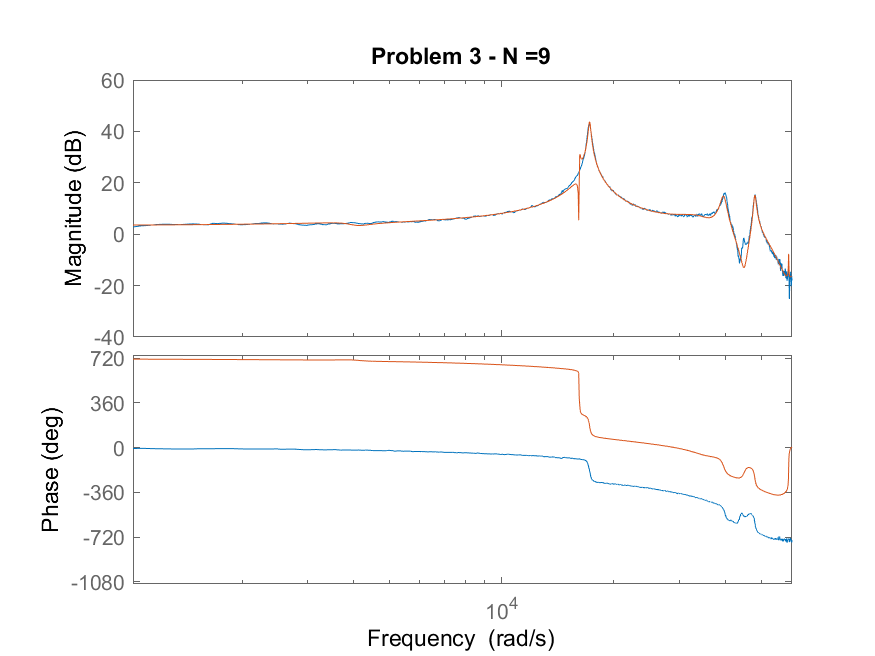
\includegraphics[width=0.7\linewidth]{fig/MECH6325_CA1_pblm3_n=9}
			\caption{Bode Plot of the measured response versus the 9th order least-squares estimated system.}
			\label{fig:pblm3_n=9}
		\end{figure}

		\begin{figure}[h]
			\centering
			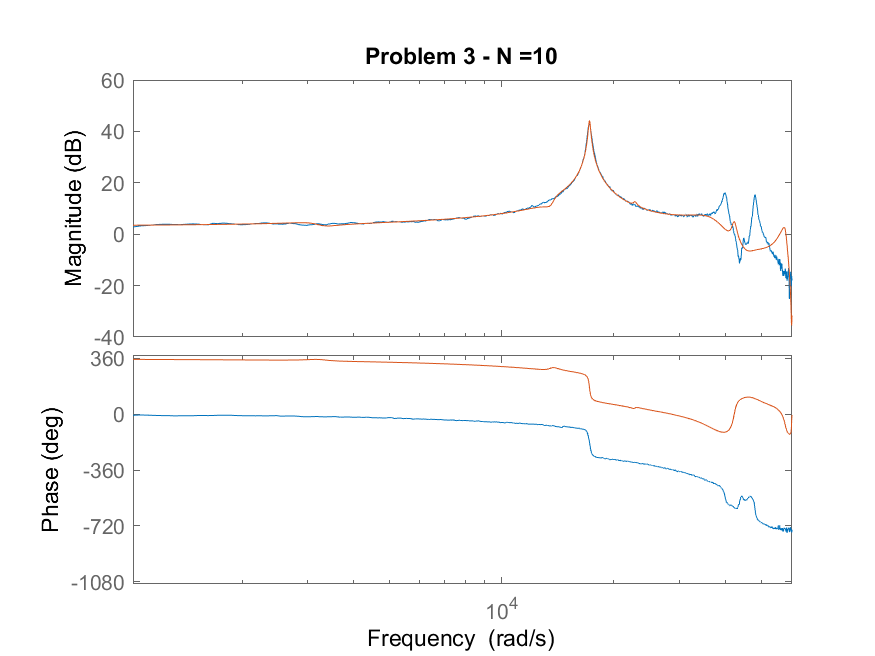
\includegraphics[width=0.7\linewidth]{fig/MECH6325_CA1_pblm3_n=10}
			\caption{Bode Plot of the measured response versus the 10th order least-squares estimated system.}
			\label{fig:pblm3_n=10}
		\end{figure}

		\begin{figure}[h]
			\centering
			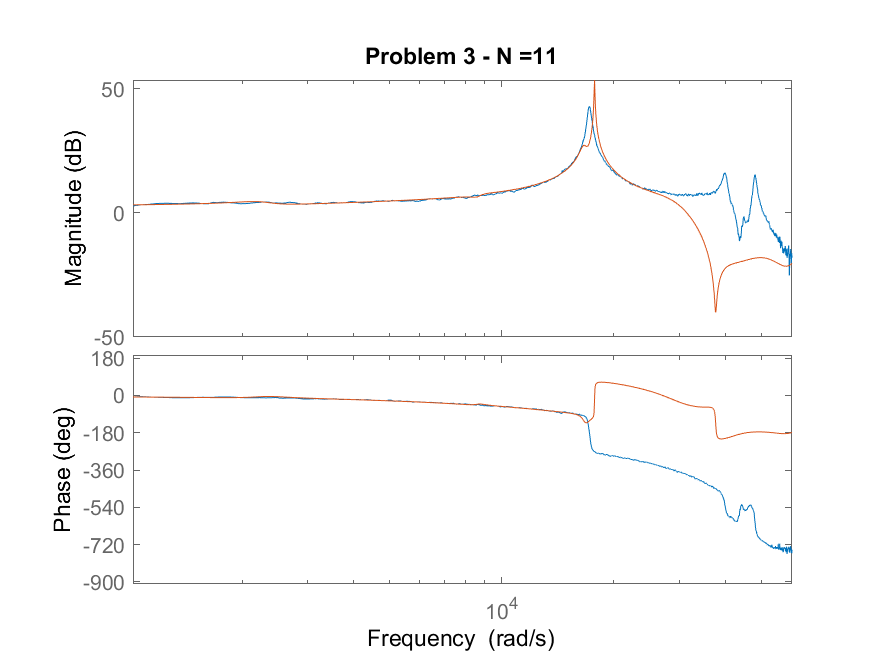
\includegraphics[width=0.7\linewidth]{fig/MECH6325_CA1_pblm3_n=11}
			\caption{Bode Plot of the measured response versus the 11th order least-squares estimated system.}
			\label{fig:pblm3_n=11}
		\end{figure}

		\begin{figure}[h]
			\centering
			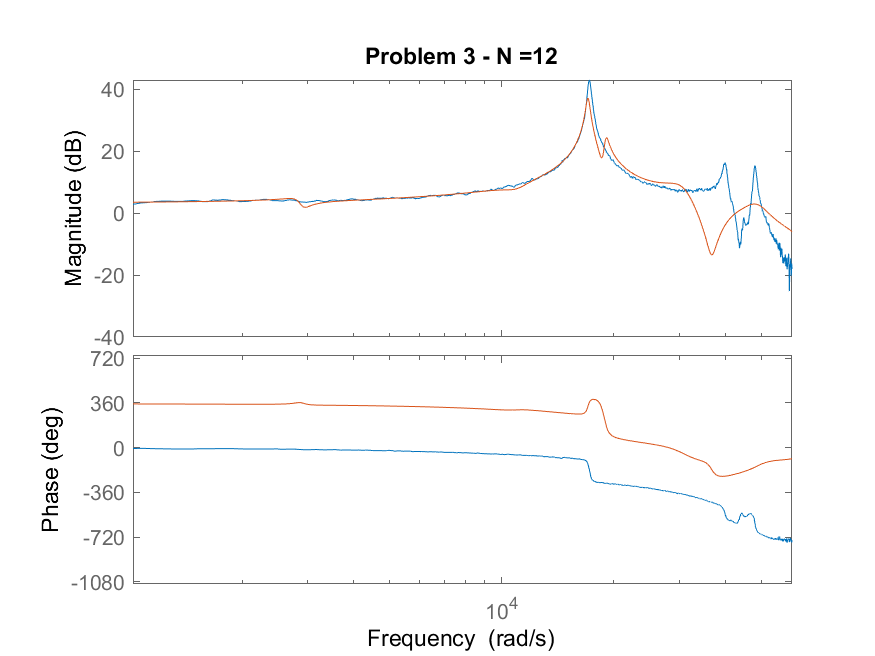
\includegraphics[width=0.7\linewidth]{fig/MECH6325_CA1_pblm3_n=12}
			\caption{Bode Plot of the measured response versus the 12th order least-squares estimated system.}
			\label{fig:pblm3_n=12}
		\end{figure}
		
		
\end{document}
